%!TEX root = draft.tex
%\newcommand{\seqPQ}{\mathsf{SeqPQ}}

\section{Distributed Linearizability}
\label{sec:distributed-lin}

Let us start our formation of specifications, histories, and linearization of CRDT. 

A distributed system contains multiple objects, and each objects is replicated on each replica. Each object has a type, which contains its method and data type. A client of a replica interact with the objects by calling the method and then obtaining the return value. Here we do not bound the number of replica identifiers and objects. 

Let $\mathbb{OBJ}$ be the set of objects and $\mathbb{R}$ be the set of replica identifiers. We consider a finite set $\mathbb{M}$ of method names; and a possibly infinite set $\mathbb{D}$ of arguments and return values, the data domain. Let $\mathbb{TYPE}$ be the set of data types, while each data type $t = (M,D)$ has a set $M \subseteq \mathbb{M}$ of methods and a data domain $D \subseteq \mathbb{D}$. Finally we have a infinite set $\mathbb{O}$ of operation identifiers, corresponding to each individual operation performed on the CRDT throughout an execution.

Without loss of generality we will consider that the methods in $\mathbb{M}$ can be separated in two disjoint sets of methods: $\mathbb{Q}$ query methods that ``has no influence on the internal state'', and $\mathbb{U}$ update methods that ``influence the internal state''. Note that some update operation can also detect some internal state. For example, a $add(a,b)$ operation of distributed list intends to put $a$ immediately after $b$, which also ensures that $b$ is in list. 

Operation labels \mbox{$m(a)\Rightarrow b$} with $m \in \mathbb{M}$ and $a,b \in \mathbb{D}$, indicate that the operation calls method $m$ with argument $a$ and its return value is $b$. When $m$ does not use the argument (resp., return value), we write $m()\Rightarrow b$ (resp., $m(a)$) instead. We define an operation $o$ to be a tuple $(\ell,i,x)$, where $\ell$ is an operation label, $i \in \mathbb{O}$ is a unique operation identifier, and $x \in \mathbb{OBJ}$ is the objects of this operation. Let $\mathbb{OP}$ be the set of operations.

\noindent {\bf Sequential Specification:} A sequential specification intends to give a sequential view of the data type, and is given as a set of sequential behaviors. However, some particular methods seem inherently non-sequential. For example, in OR-set data type, a $rem(a)$ operation only cancels the added items $a$ of the local replica. It seems quite hard to give a completely sequential explanation for it and explain it globally among replicas. To deal with such operations, we introduce an additional tuple, which are the set of operations needed for this operation. Formally, let specification alphabet $\mathbb{A} = \mathbb{OP} \cup \{ (o,s) \vert o \in \mathbb{OP}, s \subseteq \mathbb{O} \}$. Then, a sequential specification of CRDT is given as a set of sequences over specification alphabets $\mathbb{A}$. From now on, we implicitly assume that for each sequences of sequential specification, each operation has a unique operation identifier. Given a data type $t = (M,D)$, let $\mathit{specMth}(t) \subseteq M$ be the set of methods, such that in its sequential specification, only operations of $\mathit{specMth}(t)$ uses specification alphabet of the form $(o,s)$. Or we can say, $\mathit{specMth}(t)$ is the set of methods that needs specially treated, like $rem$ of OR-set. We call methods in $\mathit{specMth}(t)$ special methods, and call the arguments $s$ of $(o,s)$ special arguments.

\gp{We should add the specifications (even non-deterministic here.)}
\begin{definition}[Sequential Specification]
\label{definition:sequential specification}
A sequential specification $\mathit{spec}_s \subseteq \mathbb{A}^*$ is a set of strings over specification alphabet $\mathbb{A}$.
\end{definition}

Normally, the sequential specification is defined by the pre-condition and post-conditions. For example, for $inc$ operation of counter, it is defined as $\{ state = i \}$ $inc$ $\{ state = i+1 \}$, while $state$ is a value of integer. %Usually in sequential specification, update operations $(o,s)$ changes the state of pre-condition and ignores $s$, while query operations does not change the state of pre-condition and uses $s$. 
The detailed examples of sequential specifications are shown latter of this section. 

\noindent {\bf Distributed Specification:} Given a sequence $s$ and a set $S$ of operations, let $s \uparrow_{S}$ be the projection of $s$ over $S$. To give distributed specification, we need to give the linearization, as well as the visibility relation, and check that, for each query operation $o$, the projection of $s$ into $o$ and operations visible to $o$ is in the sequential specification. The notion of distributed specification is defined as follows:


%where $s \subseteq \mathbb{A}^*$ is a sequence of specification alphabet, and $v$ is a function that maps each item $a$ of $s$ into a subset of items before $a$ in $s$. Here $s$ essentially is the linearization of an execution, while $v$ is used to ensure each specification alphabet is correct in this sequence. %Given a sequence $s \subseteq \mathbb{A}^*$ of specification alphabets and a specification alphabets $a$, let $\mathit{itm}(s)$ be the set of specification alphabets of $s$, and $\mathit{itmBef}(s,a)$ be the set of specification alphabets of $s$ that appears before $a$, or $\emptyset$ otherwise.
%Given a sequence $s$ and a set of operations $S$, let $s \uparrow_{S}$ be the projection of $s$ over $S$. Given a sequence $s$ and an item $a$ of $s$, let $\mathit{bef}(s,a)$ contains the set of items of $s$ that appear before $a$ in $s$, as well as all the subsets of this set.

\gp{I don't really know what a Dist. Spec. is.}
\begin{definition}[Distributed Specification]
\label{definition:distributed specification}
A distributed specification $\mathit{spec}_d$ w.r.t a sequential specification $\mathit{spec}_s$ is a set of tuples $(s,f)$, such that

\begin{enumerate}[(i)]
\item $s \in \mathbb{OP}^*$ is a sequence of operations,
\item $f$ is a function that maps each operation $o$ of $s$ into a subset of operations in prefix of $o$, and
\item for each query operation $o$, $f(s) \uparrow_{ ( \{ o \} \cup f^{-1}(o))} \in \mathit{spec}_s$.
\end{enumerate}

here $f(s)$ is the sequence obtained from $s$ by replacing each $\mathit{specMth}(t)$ operation $o$ with $(o,f(o))$, while keeping other operations unchanged.
\end{definition}

Essentially, $s$ is the ilnearization of an execution, and $f$ maps each operation $o$ into the operations that are visible to $o$. It is easy to see that, as long as the sequential specification is given, its distributed specification is done. Definition \ref{definition:distributed specification} assumes that a operation $o$ of special method will use operations visible to it as its special arguments. This fits the practice of CRDT-algorithms.

The examples of sequential specifications of typical CRDT types are given below. For each object we need to consider whether it is consistent with its specification. Or we can say, in each specification we need to concern only one object. 

\begin{example}[Counter]
\label{definition:sequential specification of counter}
The sequential specification $\mathit{counter}_s$ of counter is given as follows: Let $\mathit{state}$ be a integer.

\begin{itemize}
\setlength{\itemsep}{0.5pt}
\item[-] $\{ \mathit{state} = i \}$ $\mathit{inc}$ $\{ \mathit{state} = i+1 \}$.
\item[-] $\{ \mathit{state} = i \}$ $\mathit{dec}$ $\{ \mathit{state} = i-1 \}$.
\item[-] $\{ \mathit{state} = i \}$ $\mathit{read}() \Rightarrow i$ $\{ \mathit{state} = i \}$.
\end{itemize}
\end{example}


\begin{example}[Set]
\label{definition:sequential specification of set}
The sequential specification $\mathit{set}_s$ of set is given as follows: Here we assume that each item is put into the set only once. Let $\mathit{state}$ be a set and each its element $(a,f)$ is a tuple of a data $a$ and a flag $f \in \{ \mathit{true},\mathit{false} \}$.

\begin{itemize}
\setlength{\itemsep}{0.5pt}
\item[-] $\{ \mathit{state} = S \wedge a \notin S \}$ $\mathit{add}(a)$ $\{ \mathit{state} = S \cup \{ (a,\mathit{true}) \} \}$.
\item[-] $\{ \mathit{state} = S \wedge S_1 = \{a \vert (a,\mathit{true}) \in S \} \}$ $\mathit{read}() \Rightarrow S_1$ $\{ \mathit{state} = S \}$.
\item[-] $\{ \mathit{state} = S \wedge \exists f, (a,f) \in S \}$ $\mathit{rem}(a)$ $\{ \mathit{state} = S \setminus \{ (a,f) \} \cup \{ (a,\mathit{false}) \} \}$.
\end{itemize}
\end{example}



\begin{example}[OR-Set]
\label{definition:sequential specification of or-set}
The sequential specification $\mathit{OR}$-$\mathit{Set}_s$ of OR-set is given as follows: Let $\mathit{state}$ be a set and each its element $(a,\mathit{id},f)$ is a tuple of a data $a$, a operation identifier $\mathit{id} \in \mathbb{O}$, and a flag $f \in \{ \mathit{true},\mathit{false} \}$. Note that here $(add(a),\mathit{id})$ is an operation of label $add(a)$ and identifier $\mathit{id}$. The special method of OR-set is $\mathit{rem}$.
\begin{itemize}
\setlength{\itemsep}{0.5pt}
\item[-] $\{ \mathit{state} = S  \wedge (\_,\mathit{id},\_) \notin S \}$ $(\mathit{add}(a),\mathit{id})$ $\{ \mathit{state} = S \cup \{ (a,\mathit{id},\mathit{true}) \} \}$.
\item[-] $\{ \mathit{state} = S \wedge S_1 = \{ a \vert (a,\_,\mathit{true}) \in S \} \}$ $\mathit{read}() \Rightarrow S_1$ $\{ \mathit{state} = S \}$.
\item[-] $\{ \mathit{state} = S  \wedge S_1 \subseteq \{\mathit{id} \vert (\_,\mathit{id},\_) \in S\} \}$ $((rem(a),\mathit{id}'),S_1)$ $\{ \mathit{state} = S_2  \}$. Here $S_2$ is obtained from $S$ by marking the flag of each $S_1 \uparrow_{a}$ item into $\mathit{false}$.
\end{itemize}
\end{example}


\begin{example}[Register]
\label{definition:sequential specification of register}
The sequential specification $\mathit{reg}_s$ of register is given as follows: Let $\mathit{state} \in \mathbb{D}$ be a value.
\begin{itemize}
\setlength{\itemsep}{0.5pt}
\item[-] $\{ \mathit{state} = a  \}$ $\mathit{write}(b)$ $\{ \mathit{state} = b \}$.
\item[-] $\{ \mathit{state} = a \}$ $\mathit{read}() \Rightarrow a$ $\{ \mathit{state} = a \}$.
\end{itemize}
\end{example}


\begin{example}[Multi-value Register]
\label{definition:sequential specification of multi-value register}
The sequential specification $\mathit{MVReg}_s$ of multi-value register is given as follows: Let $\mathit{state}$ be a set and each its element $(a,\mathit{id},f)$ is a tuple of a data $a$, a operation identifier $\mathit{id} \in \mathbb{O}$, and a flag $f \in \{ \mathit{true},\mathit{false} \}$. The special method of multi-value register is $\mathit{write}$.
\begin{itemize}
\setlength{\itemsep}{0.5pt}
\item[-] $\{ \mathit{state} = S \wedge S_1 \subseteq \{\mathit{id}' \vert (\_,\mathit{id}',\_) \in S\} \wedge (\_,\mathit{id},\_) \notin S \}$ $((write(b),id),S_1)$ $\{ \mathit{state} = S_2 \}$. Here $S_2$ is obtained from $S$ by marking each $S_1$ item with $\mathit{false}$, and then insert $(b,id,\mathit{true})$.
%\item[-] $\{ \mathit{state} = S \wedge \forall x \in S_1, (b,x,\mathit{true}) \in S_1 \vee (b,x,\mathit{false}) \in S_1 \}$ $((write(b),id),S_1)$ $\{ \mathit{state} = S_2 \}$. Here $S_2$ is obtained from $S$ by mark each $(b,x)$ with $\mathit{false}$, and then insert $(b,id,\mathit{true})$.
\item[-] $\{ \mathit{state} = S \wedge S_1 = \{ a \vert (a,\_,\mathit{true}) \in S \} \}$ $read() \Rightarrow S_1$ $\{ \mathit{state} = S \}$.
\end{itemize}
\end{example}


\begin{example}[List with add-after interface]
\label{definition:sequential specification of list with add-after interface}
The sequential specification $\mathit{list}_s$ of list is given as follows: Let $\mathit{state}$ be a sequence, where each item is a tuple $(a,f)$ with data $a$ and flag $f \in \{ \mathit{true},\mathit{false} \}$.
\begin{itemize}
\setlength{\itemsep}{0.5pt}
\item[-] $\{ \mathit{state} = (a_1,f_1) \cdot \ldots \cdot (a_n,f_n) \wedge l \leq n \wedge b \notin \{ a_1, \ldots, a_n \} \}$ $add(b,a_l)$ $\{ \mathit{state} = (a_1,f_1) \cdot \ldots \cdot (a_l,f_l) \cdot (b,\mathit{true}) \cdot (a_{l+1},f_{l+1}) \cdot \ldots \cdot (a_n,f_n) \}$.
\item[-] $\{ \mathit{state} = (a_1,f_1) \cdot \ldots \cdot (a_n,f_n) \wedge S = \{ a \vert (a,\mathit{true}) \in \mathit{state} \} \wedge l = a_1 \cdot \ldots \cdot a_n \uparrow_{S} \}$ $read() \Rightarrow l$ $\{ \mathit{state} = (a_1,f_1) \cdot \ldots \cdot (a_n,f_n) \}$.
\end{itemize}
\end{example}


\noindent {\bf Distributed Linearizability:} As customary, to capture the notion of client-observable effects of an execution over a CRDT, we will define the notion of \emph{history}. A history contains a set of operations, and the order in which they were effected in each replica. Formally, a history $h$ is a tuple of the form $h = (Op,\mathit{ro})$ where $Op$ is a set of operations, and $\mathit{ro}$ is a union of transitive, irreflexive and total orders of identifiers of $O$.

%Formally, a history $h$ is a tuple of the form $h = (O,\mathit{lab},\mathit{ro})$ where $O$ is a set of operation identifiers, $\mathit{lab}$ is a function that maps each operation identifiers of $O$ into a operation label, and $\mathit{ro}$ is a union of transitive, irreflexive and total orders of $O$.

A history is single-object, if it contains operations of a single object. A history is multi-object, if it contains operations of multiple object. A multi-object history $h$ is linearizable w.r.t specification of its objects, if we can found the linearization of operations of $h$ and a visibility relation $\mathit{vis}$ of $h$, such that for each objects $x$, the projection of $h$ and $\mathit{vis}$ over operations of $x$ are in its distributed specification.

%A history $h$ is distributed linearizable w.r.t a distributed specification $\mathit{spec}$, if we can find $(s,f) \in \mathit{spec}_d$ and a visibility relation $\mathit{vis}$ of $h$, such that $\mathit{vis}$ and $f$ are consistent. Formally,

\begin{definition}[Distributed Linearizability]
\label{definition:distributed linearizability} 

Let $h = (O,\mathit{ro})$ be a multi-object history and $\mathit{Obj}$ be the set of objects of $h$. $h$ is distributed linearizable w.r.t specifications of $\mathit{Obj}$, if there exists a acyclic visibility relation $\mathit{vis} \subseteq O \times O$ with $\mathit{ro} \subseteq \mathit{vis}$, and for each object $x \in \mathit{Obj}$: there exists $(s,f)$ in distributed specification of $x$ and , such that

\begin{enumerate}[(i)]
\item The set of operations of $s$ is the set of operations of $h \uparrow_{x}$,   
\item The order obtained by projection $\mathit{vis}$ over operations of $x$ is consistent with $s$,
\item For each operation $o_1$ of $h \uparrow_{x}$, $f(o_1) = \{ o_2 \vert o_2 \in h \uparrow_{x} \wedge (o_2,o_1) \in \mathit{vis} \}$. 
\end{enumerate} 

We say that $h$ is distributed linearizable if $h$ is distributed linearizable w.r.t specifications of its objects. A set $H$ of histories of multi-objects is distributed linearizable, if each of its history is. 
\end{definition}


\gpn{Definition of CRDT-Linearizablity correctness.}

In the following we show an example of distributed linearizable history and an example of non-distributed linearizable history. Both example contains only one object. Since the function $f$ of $(s,f)$ in distributed specification can be obtained from the visibility relation, here we draw the visibility relation and readers could easily obtain the function $f$.

\figurename~\ref{fig:a distributed linearizable history} is an example of a distributed linearizable history of OR-set. Its linearization is $\mathit{add}(0)_1 \cdot \mathit{add}(1)_2 \cdot \mathit{rem}(0) \cdot \mathit{add}(1)_1 \cdot \mathit{add}(0)_2 \cdot \mathit{rem}(1) \cdot \mathit{read}()_1 \Rightarrow \{0,1\} \cdot \mathit{read}()_2 \Rightarrow \{0,1\}$. The special arguments of $\mathit{rem}(0)$ is the identifiers of $\{ \mathit{add}(0)_1, \mathit{add}(1)_2 \}$, and the special arguments of $\mathit{rem}(1)$ is the identifiers of $\{ \mathit{add}(1)_1, \mathit{add}(0)_2 \}$.

\figurename~\ref{fig:a non-distributed linearizable history} is an example of a non-distributed linearizable history of OR-set. Here we can not validate $\mathit{read}() \Rightarrow \{ 1 \}$. 

\begin{figure}[t]
  \centering
  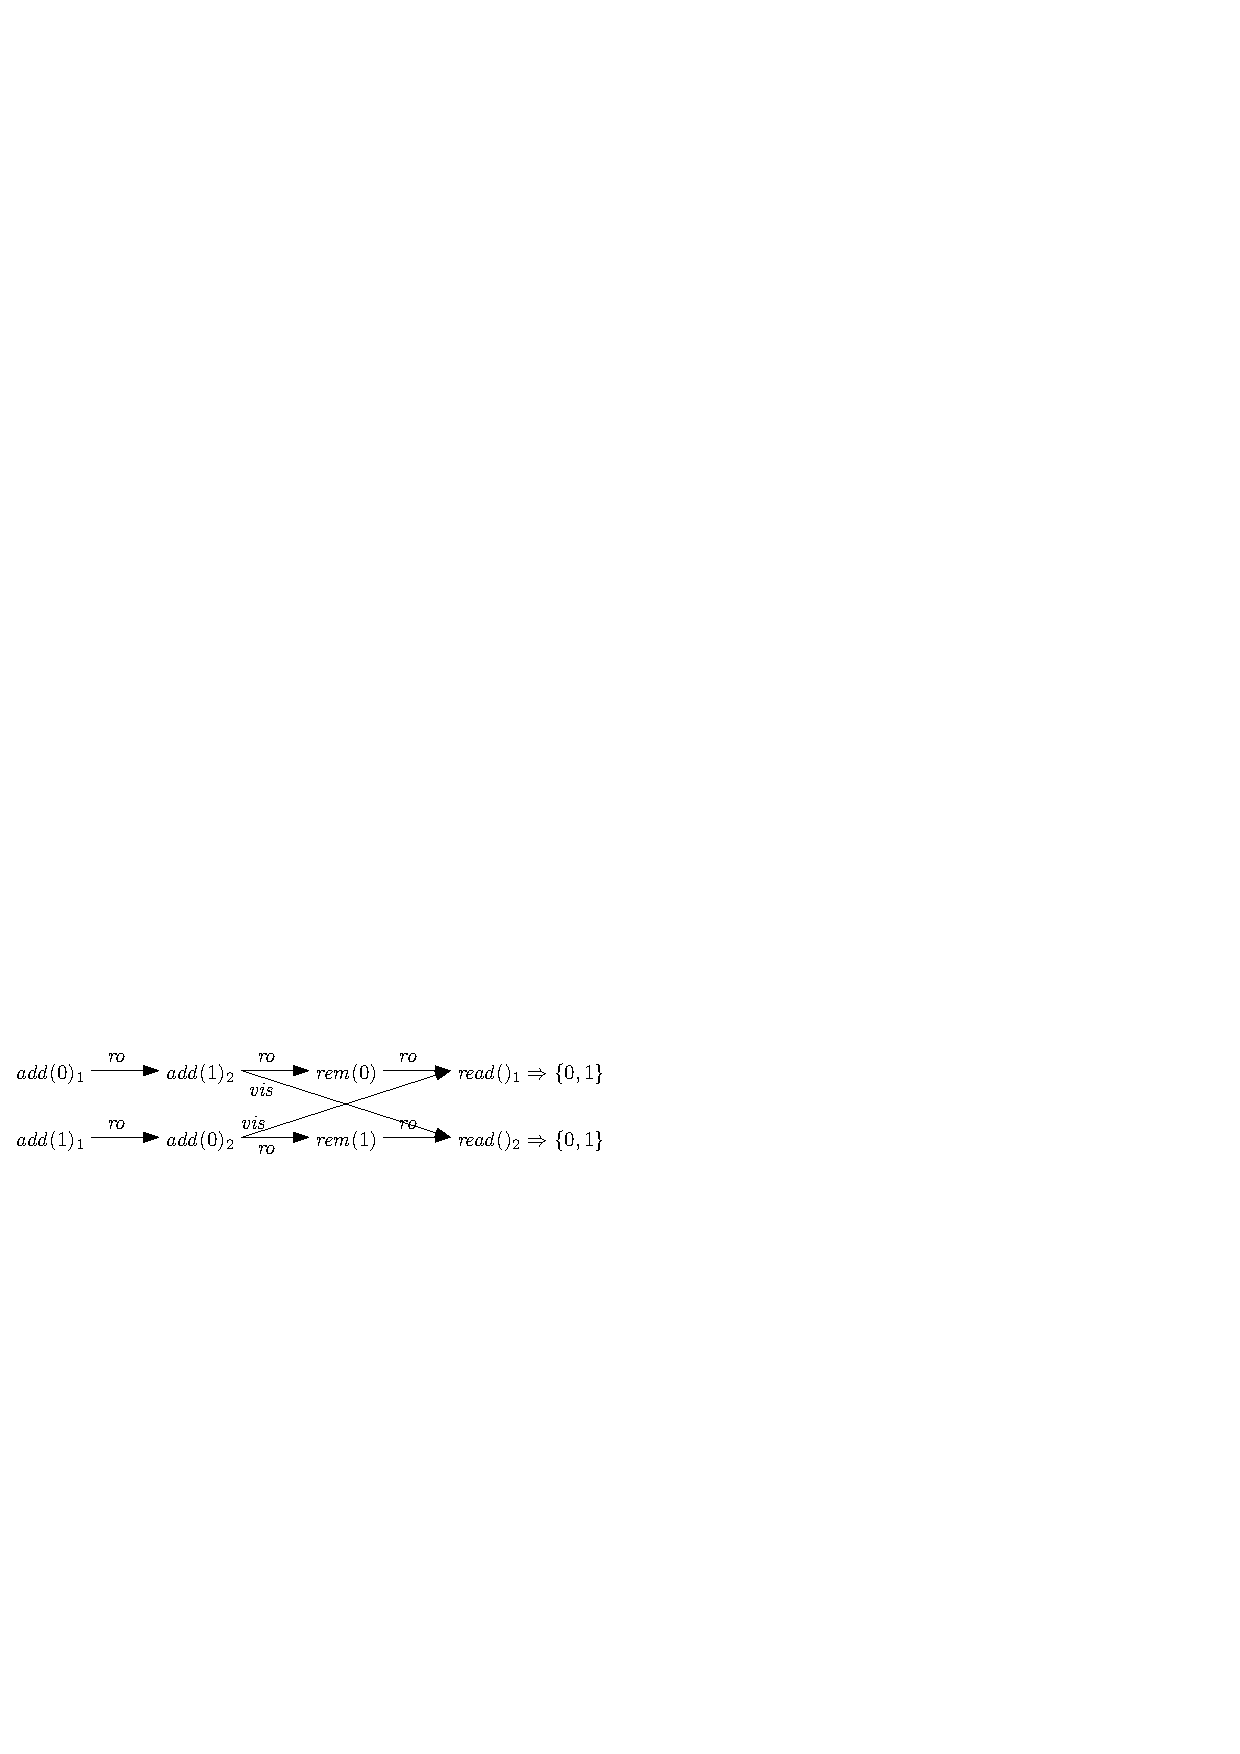
\includegraphics[width=0.7 \textwidth]{figures/PIC-Example-LinHis.pdf}
%\vspace{-10pt}
  \caption{A distributed linearizable history. Here subscript of $\mathit{add}(0)_1$ is used to distinguish different $\mathit{add}(0)$ operations.}
  \label{fig:a distributed linearizable history}
\end{figure}



\begin{figure}[t]
  \centering
  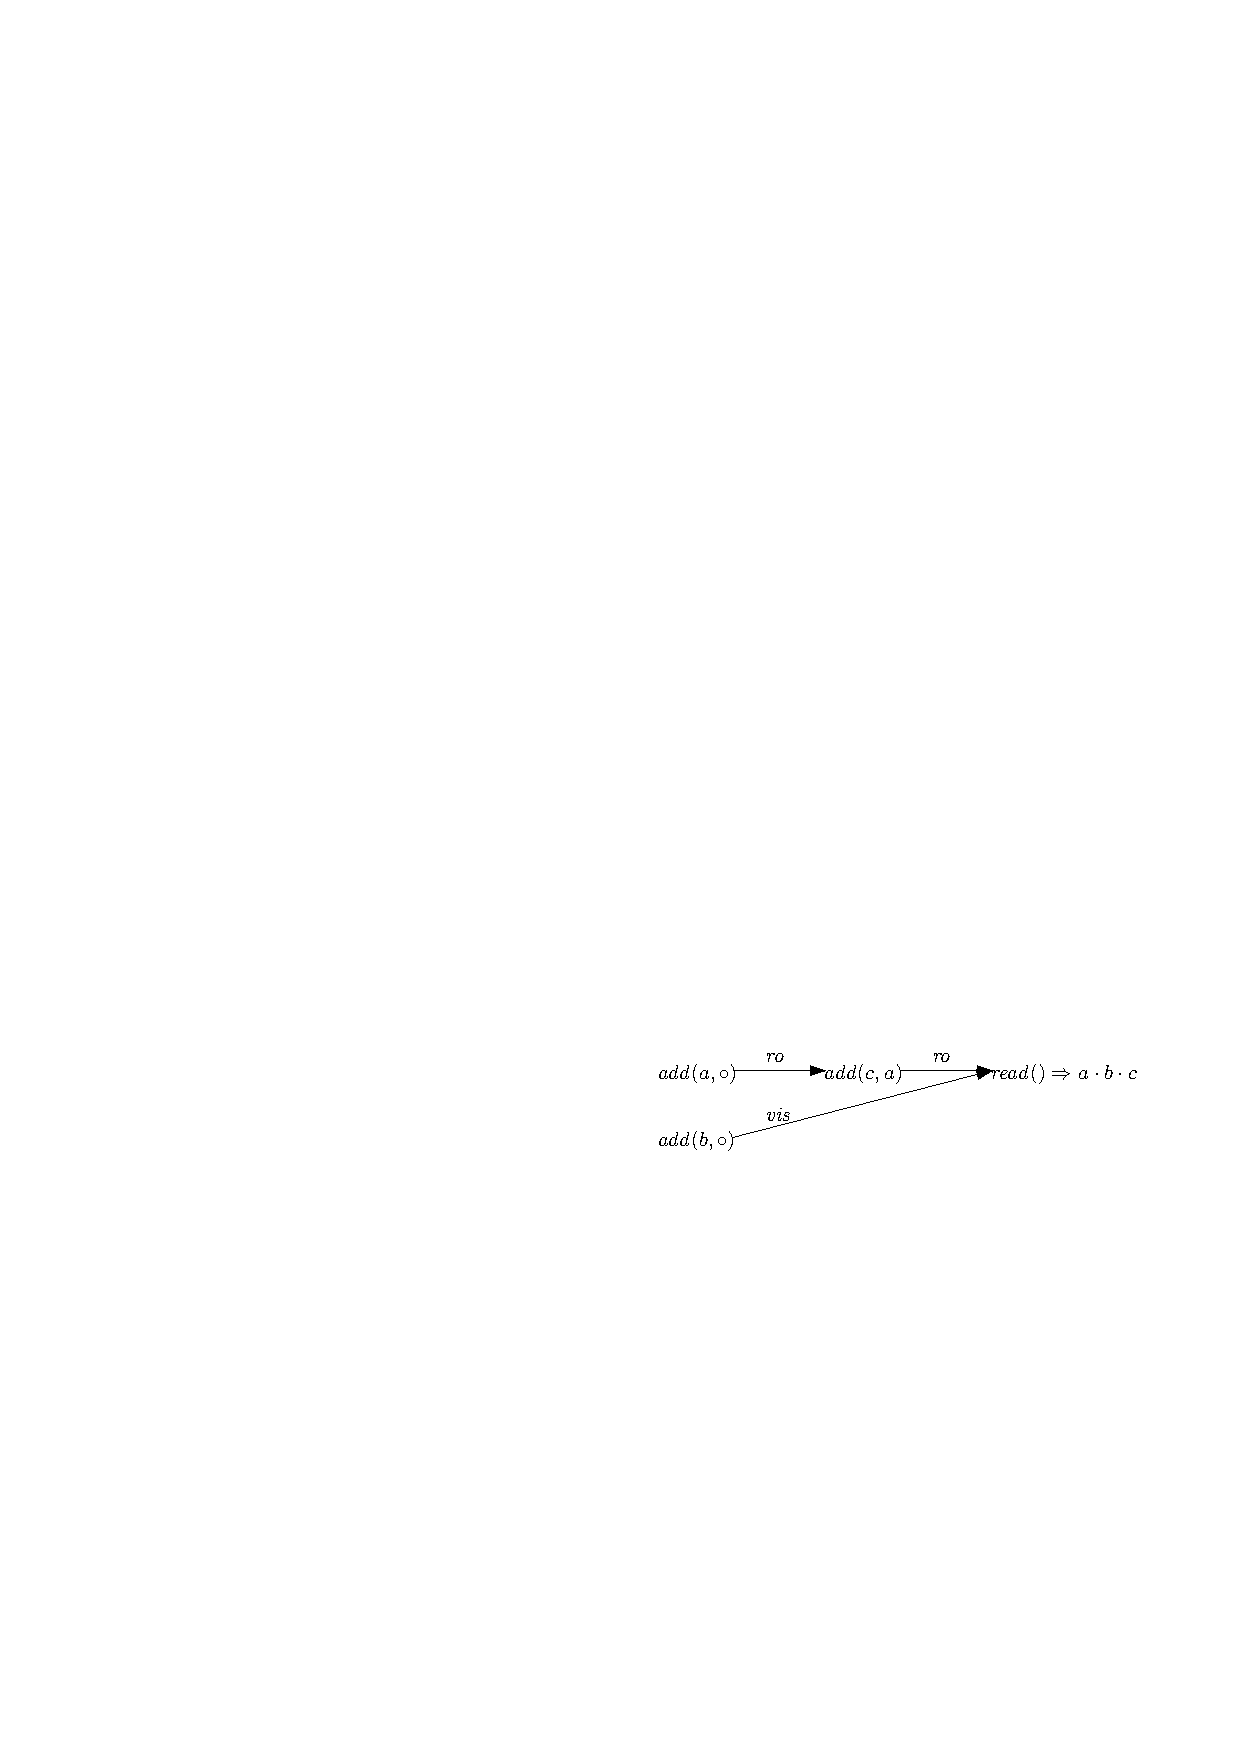
\includegraphics[width=0.6 \textwidth]{figures/PIC-Example-NonLinHis.pdf}
%\vspace{-10pt}
  \caption{A non-distributed linearizable history.}
  \label{fig:a non-distributed linearizable history}
\end{figure}


%%% Local Variables:
%%% mode: latex
%%% TeX-master: "draft"
%%% End:
